\documentclass{article}

\usepackage[margin=3cm]{geometry}
\usepackage{amsmath}
\usepackage{amssymb}
\usepackage{graphicx}

\title{\Large\bfseries CS 477: Formal Software Development Methods \\
Fall 2016 \\
Homework 1}
\author{Chiao Hsieh, chsieh16@illinois.edu}

\begin{document}
\maketitle

\begin{enumerate}
\item \textbf{[20 points]}

Consider a formal syntax for well-formed propositional logic give as:
\[
    Formulas\ \alpha, \beta ::= p_i \mid \neg\alpha \mid \alpha\lor\beta \mid \alpha\land\beta
\]
where \(P = \{p_0, p_1, p_2, \cdots\}\) is an infinite set of propositions, and where \(i\in \mathbb{N}\)

For any formula \(\alpha\), let the dual of \(\alpha\)
be defined as follows, inductively:
\[
\begin{array}{l}
Dual(p) = \neg p \text{ for every } p \in \mathcal{P} \\
Dual(\neg\alpha) = \neg Dual(\alpha) \text{ for every formula} \\
Dual(\alpha\lor\beta) = Dual(\alpha) \land Dual(\beta) \text{ for any two formulas }\alpha, \beta \\
Dual(\alpha\land\beta) = Dual(\alpha) \lor Dual(\beta) \text{ for any two formulas }\alpha, \beta
\end{array}
\]

Prove that for any model \(M\) and any formula \(\alpha\),
\[
  M \models \alpha\ \mathit{iff}\ M \not\models Dual(\alpha)
\]

You must prove this formally by structural induction over formulas
(using the inductive definition of \(\models\)  presented in class).
Vague arguments or hand-waving arguments will fetch close to zero points.
Wrong boring proofs are fine
(don't try to be concise, try to be correct and formal first).

\medskip
Ans.
\medskip

\textbf{Base Step:}
\[
\begin{array}{rll}
	         & M \models \neg p \ \mathit{iff}\ M \not\models p & \text{(definition of \(\neg\))}\\
	\implies & M \models Dual(p)\ \mathit{iff}\ M \not\models p & \because Dual(p) = \neg p\\
	\implies & M \not\models Dual(p)\ \mathit{iff}\ M \models p\\
\end{array}
\]

Hence, it holds for any atomic proposition \(p\).

\textbf{Inductive Step:}

For negation,
assuming \(M \models \alpha\ \mathit{iff}\ M \not\models Dual(\alpha)\) is valid for \(\alpha\),
\[
\begin{array}{rll}
   & M \models \alpha\ \mathit{iff}\ M \not\models Dual(\alpha) & \text{(induction hypothesis)}\\
 \implies & M \not\models \alpha\ \mathit{iff}\ M \models Dual(\alpha) \\
 & M \models \neg \alpha \ \mathit{iff}\ M \not\models \alpha & \text{(definition of \(\neg\))}\\
 \implies & M \models \neg \alpha \ \mathit{iff}\ M \models Dual(\alpha) \\
 & M \not\models \neg Dual(\alpha)\ \mathit{iff}\ M \models Dual(\alpha)  & \text{(definition of \(\neg\))}\\
 \implies & M \models \neg \alpha \ \mathit{iff}\ M \not\models \neg Dual(\alpha) \\
 \implies & M \models \neg \alpha \ \mathit{iff}\ M \not\models Dual(\neg \alpha) & \because Dual(\neg\alpha) = \neg Dual(\alpha)
\end{array}
\]

For disjunction,
assuming \(M \models \alpha\ \mathit{iff}\ M \not\models Dual(\alpha)\) 
and \(M \models \beta\ \mathit{iff}\ M \not\models Dual(\beta)\) are valid for \(\alpha\) and \(\beta\),
\[
\begin{array}{rll}

   & M \not\models \neg(\neg Dual(\alpha)\lor \neg Dual(\beta))\ \mathit{iff}\ M \models \neg Dual(\alpha)\lor \neg Dual(\beta)  & \text{(definition of \(\neg\))}\\
 \implies & \multicolumn{2}{l}{M \not\models Dual(\alpha)\land Dual(\beta)\ \mathit{iff}\ M \models \neg Dual(\alpha)\lor \neg Dual(\beta) \qquad \because \alpha\land\beta = \neg (\neg\alpha \lor \neg\beta)}\\
 \implies & \multicolumn{2}{l}{M \not\models Dual(\alpha\lor\beta)\ \mathit{iff}\ M \models \neg Dual(\alpha)\lor \neg Dual(\beta) \qquad \because Dual(\alpha\lor\beta) = Dual(\alpha)\land Dual(\beta)}\\
 and & M \models \neg Dual(\alpha)\lor \neg Dual(\beta)\ \mathit{iff}\ (M \models \neg Dual(\alpha) \ \mathit{or}\ M \models \neg Dual(\beta)) & \text{(definition of \(\lor\))}\\
 \implies & M \not\models Dual(\alpha\lor\beta)\ \mathit{iff}\ (M \models \neg Dual(\alpha) \ \mathit{or}\ M \models \neg Dual(\beta)) \\
 and & M \models \neg Dual(\alpha) \ \mathit{iff}\ M \not\models Dual(\alpha) & \text{(definition of \(\neg\))}\\
 \implies & M \not\models Dual(\alpha\lor\beta)\ \mathit{iff}\ (M \not\models Dual(\alpha) \ \mathit{or}\ M \not\models Dual(\beta)) \\
 and & M \models \alpha\ \mathit{iff}\ M \not\models Dual(\alpha) & \text{(induction hypothesis)}\\
 and & M \models \beta \ \mathit{iff}\ M \not\models Dual(\beta)  & \text{(induction hypothesis)}\\
 \implies & M \not\models Dual(\alpha\lor\beta)\ \mathit{iff}\ (M \models \alpha \ \mathit{or}\ M \models \beta) \\
 and & M \models \alpha\lor\beta\ \mathit{iff}\ (M \models \alpha \ \mathit{or}\ M \models \beta) & \text{(definition of \(\lor\))}\\
 \implies & M \not\models Dual(\alpha\lor\beta)\ \mathit{iff}\ M \models \alpha\lor\beta \\
\end{array}
\]

For conjunction,
assuming \(M \models \alpha\ \mathit{iff}\ M \not\models Dual(\alpha)\) 
and \(M \models \beta\ \mathit{iff}\ M \not\models Dual(\beta)\) are valid for \(\alpha\) and \(\beta\),
\[
\begin{array}{rll}
   & M \not\models \alpha\ \mathit{iff}\ M \models Dual(\alpha) & \text{(induction hypothesis)}\\
   & M \not\models \beta \ \mathit{iff}\ M \models Dual(\beta)  & \text{(induction hypothesis)}\\
   & M \models Dual(\alpha)\lor Dual(\beta)\ \mathit{iff}\ (M \models Dual(\alpha) \ \mathit{or}\ M \models Dual(\beta))  & \text{(definition of \(\lor\))}\\
 \implies & M \models Dual(\alpha)\lor Dual(\beta)\ \mathit{iff}\ (M \not\models \alpha \ \mathit{or}\ M \not\models \beta)\\
 \implies & \multicolumn{2}{l}{M \models Dual(\alpha\land\beta)\ \mathit{iff}\ (M \not\models \alpha \ \mathit{or}\ M \not\models \beta) \qquad \because Dual(\alpha\land\beta) = Dual(\alpha)\lor Dual(\beta)}\\
 and & M \models \neg \alpha \ \mathit{iff}\ M \not\models \alpha & \text{(definition of \(\neg\))}\\
 \implies & M \models Dual(\alpha\land\beta)\ \mathit{iff}\ (M \models \neg\alpha \ \mathit{or}\ M \models \neg\beta)\\
 and & M \models \neg\alpha\lor\neg\beta\ \mathit{iff}\ (M \models \neg\alpha \ \mathit{or}\ M \models \neg\beta)  & \text{(definition of \(\lor\))}\\
 \implies & M \models Dual(\alpha\land\beta)\ \mathit{iff}\ M \models \neg\alpha \lor \neg\beta\\
 and & M \not\models \neg(\neg\alpha \lor \neg\beta) \ \mathit{iff}\ M \models \neg\alpha \lor \neg\beta & \text{(definition of \(\neg\))}\\
 \implies & M \models Dual(\alpha\land\beta)\ \mathit{iff}\ M \not\models \neg(\neg\alpha \lor \neg\beta)\\
 \implies & \multicolumn{2}{l}{M \models Dual(\alpha\land\beta)\ \mathit{iff}\ M \not\models \alpha \land \beta \qquad \because \alpha\land\beta = \neg (\neg\alpha \lor \neg\beta)}
\end{array}
\]


\item \textbf{[10+10+10+10=40 points]}

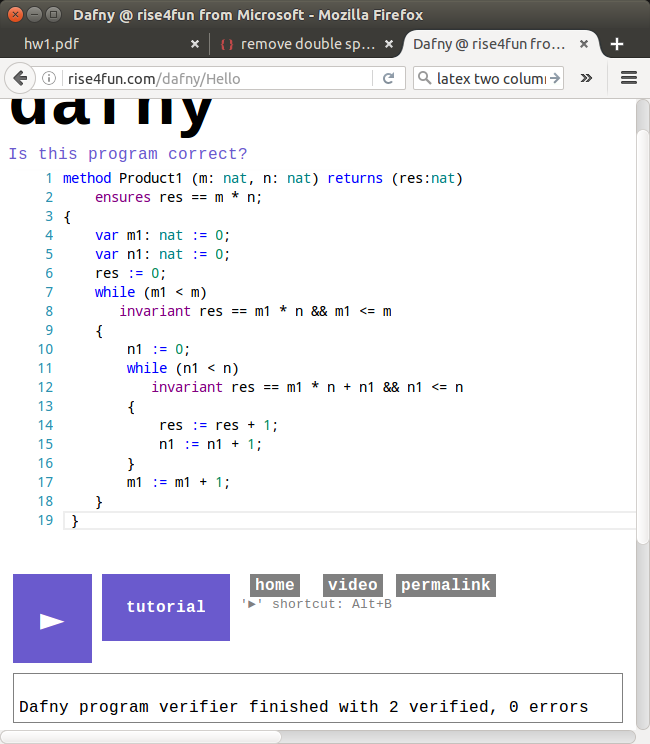
\includegraphics[width=.4\textwidth]{product1.png}
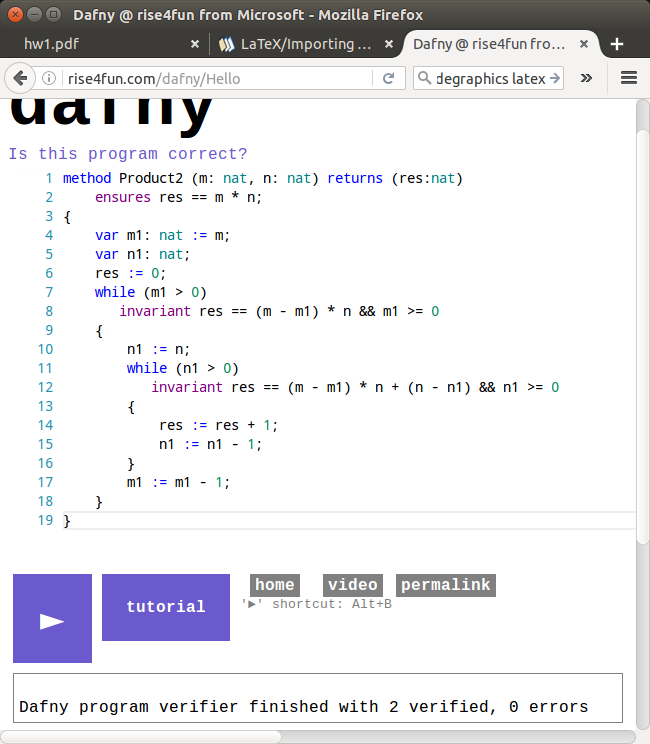
\includegraphics[width=.4\textwidth]{product2.png}

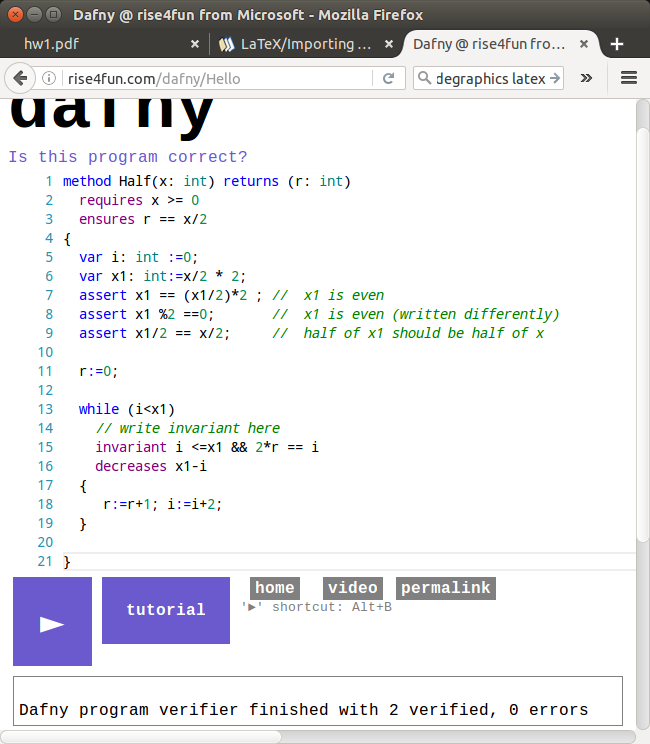
\includegraphics[width=.4\textwidth]{half.png}
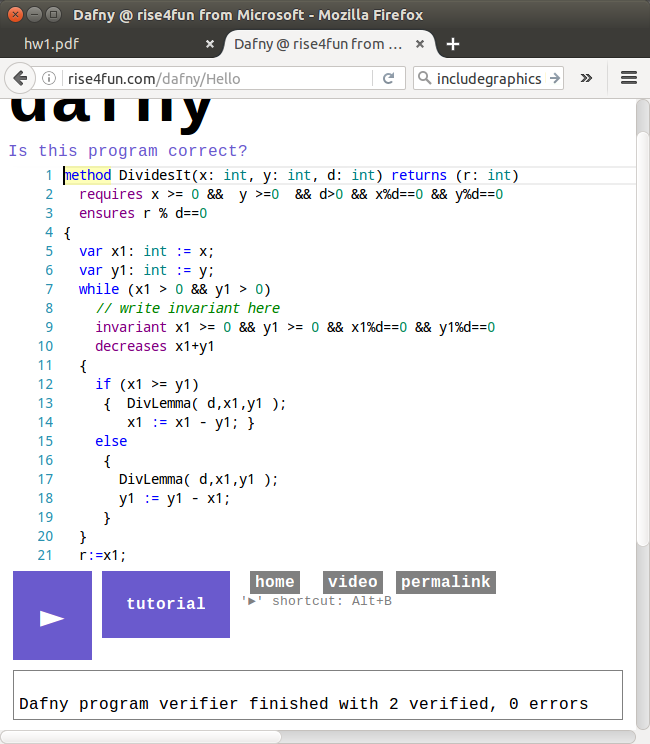
\includegraphics[width=.4\textwidth]{dividesit.png}

\item \textbf{[15+5=20 points]}

Verification Condition 1:
\[
((0 \leq x \land 0 \leq y) \land (r_0 = 2*x \land n_0 = y)) \Rightarrow (r_0 = 2*x+y-n_0 \land 0 \leq n_0)
\]

Verification Condition 2:
\[
((r_0 = 2*x+y-n_0 \land 0 \leq n_0) \land (n_0 > 0 \land r_1 = r_0 + 1 \land n_1 = n_0 - 1)) \Rightarrow (r_1 = 2*x+y-n_1 \land 0 \leq n_1)
\]

Verification Condition 3:
\[
((r_0 = 2*x+y-n_0 \land 0 \leq n_0) \land \neg(n_0 > 0)) \Rightarrow (r_0 = 2*x+y)
\]

Invalid Verification Condition 3:
\[
((r_0 = 2*x+y-n_0) \land \neg(n_0 > 0)) \Rightarrow (r_0 = 2*x+y)
\]
It's invalid since the solver cannot prove \(n_0\) is 0.



\end{enumerate}

\end{document}